\paragraph{IUP01.1 Recuperar contraseña} \hspace{1cm}\\ 
\label{pant:IUP01.1} 

\textbf{\textcolor[rgb]{0, 0, 0.545098}{Objetivo}}\\
Esta pantalla permite al Practicante recuperar su contraseña para posteriormente iniciar sesión en la herramienta, solicitando que se le envíe la contraseña al correo registrado.\\

\textbf{\textcolor[rgb]{0, 0, 0.545098}{Diseño}}\\
En la figura \ref{fig:IUP01.1} se muestra la pantalla \nameref{fig:IUP01.1}, por medio de la cual el Entrenador deberá ingresar la información requerida para recuperar su contraseña.\\

En la parte inferior se encuentran los botones de Enviar Contraseña y Cancelar.

\begin{figure}[H]
	\centering
		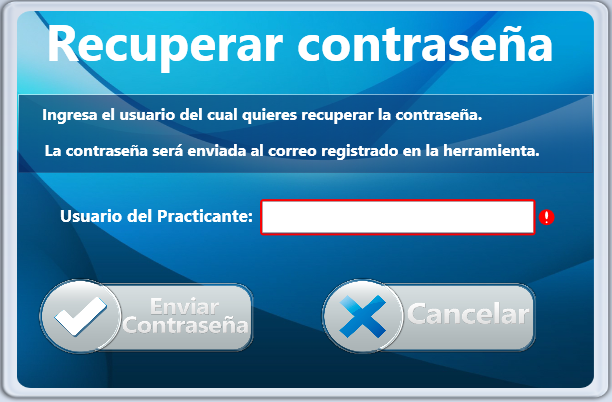
\includegraphics[scale=0.8]{./Figuras/Pantallas/IUP01_1Recuperar_contrasena}
	\caption{IUP01.1 Recuperar contraseña}
	\label{fig:IUP01.1}
\end{figure}

\textbf{\textcolor[rgb]{0, 0, 0.545098}{Entradas}}\\
En esta pantalla el Entrenador deberá capturar la siguiente información:

\begin{itemize}
	\item El usuario del Practicante.
\end{itemize}
\vspace{1em}

\textbf{\textcolor[rgb]{0, 0, 0.545098}{Comandos}}
\begin{itemize}
	\item \textbf{\textcolor[rgb]{0, 0, 0.545098}{Enviar contraseña:}}  Realiza las validaciones necesarias y envía la contraseña al correo electrónico registrado del Practicante.	
\end{itemize}

\vspace{1em}

\textbf{\textcolor[rgb]{0, 0, 0.545098}{Mensajes}}\\
	
\textbf{\nameref{msj:MSG03}}: Se muestra en la pantalla \nameref{pant:IUP01.1} indicando que la contraseña registrada ha sido enviada al correo ingresado de manera exitosa.\\

\textbf{\nameref{msj:MSG12}}: Se muestra en la pantalla \nameref{pant:IUE01} cuando el Entrenador no haya ingresado datos a los campos obligatorios.\\

\textbf{\nameref{msj:MSG13}}: Se muestra en pantalla cuando el Practicante haya ingresado alguno de los datos de manera incorrecta.\\

\clearpage